\documentclass{article}
\usepackage{graphicx} % Required for inserting images
\usepackage{bm}
\usepackage{tikz}
\usepackage{amsfonts}
\usepackage{amssymb}
\usepackage{amsmath}





\title{Quivira Math}
\date{September 2026}

\begin{document}

\maketitle

\section{Establishing Euler-Lagrange equations formally}
Let us consider a configuration space defined by $q_h$, $h = 1,\ldots,N$, also captured in vector form by $\bm q$. Introducing the Lagrangian:
$$
\mathcal L(\bm q, \dot{\bm q})
$$
and the action:
$$
S \triangleq \int_0^T \mathcal L(\bm q, \dot{\bm q})\,dt
$$
we want to use calculus of variations to find the $\bm q(t)$ that result in a minimal action. In essence we want:
$$
\min_{\bm q\in \mathcal Q} S  \triangleq
\min_{\bm q\in \mathcal Q}\int_0^T \mathcal L(\bm q, \dot{\bm q})\,dt
$$
where $\mathcal Q$ is the functional space containing all possible trajectories, with fixed endpoints. If $\overline{\bm q}(t)$ denotes a stationary trajectory, a perturbed trajectory is written as $\bm q(t)=\overline{\bm q}(t)+\delta\bm q(t)$, where the variations satisfy the boundary conditions $\delta \bm q(0) = \delta \bm q(T) = \bm 0$.

\begin{figure}[tb]
\centering
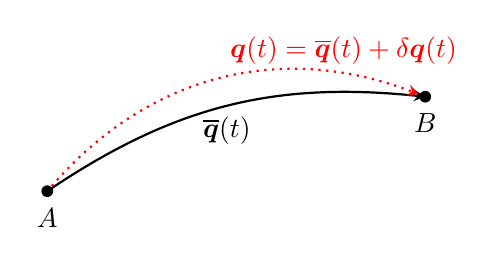
\begin{tikzpicture}[>=stealth,scale=1.2]
  % Nominal trajectory
  \draw[thick,->] (0,0) node[circle,fill,inner sep=1.5pt,label=below:$A$] (A) {}
    to[bend left=20] node[midway,below] {$\overline{\bm q}(t)$} (4,1) node[circle,fill,inner sep=1.5pt,label=below:$B$] (B) {};

  % Perturbed trajectory
  \draw[thick,dotted,red,->] (A) to[bend left=35] node[midway, right, yshift=10pt] {$\bm q(t) = \overline{\bm q}(t) + \delta \bm q(t)$} (B);
\end{tikzpicture}
\caption{Nominal trajectory $\overline{\bm q}(t)$ (solid) and perturbed trajectory $\bm q(t)=\overline{\bm q}(t)+\delta \bm q(t)$ (dotted, red) from $A$ to $B$. Note that $\delta \bm q(0) = \delta \bm q(T) = \bm 0$.}
\label{fig:trajectory}
\end{figure}
\noindent
The first variation of the Lagrangian $\delta\mathcal L$, evaluated along $\overline{\bm q}(t)$, is, to first order in $\delta\bm q$:
$$
\delta \mathcal L =
\left.
\frac{d}{d\varepsilon}
\mathcal L\left(
\overline{\bm q} + \varepsilon\delta \bm q,
\dot{\overline{\bm q}} + \varepsilon\delta\dot{\bm q}
\right)
\right|_{\varepsilon=0}
=
\frac{\partial \mathcal L}{\partial \bm q}\delta\bm q
+
\frac{\partial \mathcal L}{\partial \dot{\bm q}}\delta\dot{\bm q}.
$$
Here and below, the partial derivatives of $\mathcal L$ are evaluated at $(\overline{\bm q},\dot{\overline{\bm q}})$.
We now require the first variation of the action $\delta S$ to vanish:

\begin{align*}
\delta S
&= \int_0^T
\left(
\frac{\partial \mathcal L}{\partial \bm q}\,\delta\bm q
+
\frac{\partial \mathcal L}{\partial \dot{\bm q}}\,
\delta\dot{\bm q}
\right)\,dt \\
&= \int_0^T
\frac{\partial \mathcal L}{\partial \bm q}\,\delta\bm q\,dt
+
\int_0^T
\frac{\partial \mathcal L}{\partial \dot{\bm q}}\,
\frac{d}{dt}\left(\delta\bm q\right)\,dt \\
&= \int_0^T
\frac{\partial \mathcal L}{\partial \bm q}\,\delta\bm q\,dt
+
\left.
\frac{\partial \mathcal L}{\partial \dot{\bm q}}\,
\delta\bm q
\right|_0^T
-
\int_0^T
\frac{d}{dt}\left(
\frac{\partial \mathcal L}{\partial \dot{\bm q}}
\right)
\delta\bm q\,dt \\
&= \int_0^T
\left[
\frac{\partial \mathcal L}{\partial \bm q}
-
\frac{d}{dt}\left(
\frac{\partial \mathcal L}{\partial \dot{\bm q}}
\right)
\right]
\delta\bm q\,dt
= 0.
\end{align*}
The boundary term vanishes because $\delta\bm q(0)=\delta\bm q(T)=\bm 0$. Since $\delta\bm q$ is otherwise arbitrary, the Euler--Lagrange equations follow:
$$
\boxed{
\frac{d}{dt}\left(
\frac{\partial \mathcal L}{\partial \dot{\bm q}}
\right)
-
\frac{\partial \mathcal L}{\partial \bm q}
=
\bm 0.}
$$

\section{Adding holonomic constraints}
Let us now assume that the configuration space introduced above, of dimension $N$, is restricted by $M<N$ holonomic, time-independent constraints:
$$
\bm F(\bm q)=\bm 0
$$
where $\bm F(\bm q)\in\mathbb R^M$. We can account for these constraints by introducing a vector of time-dependent Lagrange multipliers $\bm\lambda(t)\in\mathbb R^M$ and defining the constrained action:
$$
\widetilde{S}
=
\int_0^T
\left[
\mathcal L(\bm q,\dot{\bm q})
+
\bm\lambda(t)\cdot\bm F(\bm q)
\right]\,dt.
$$
The multipliers must be functions of time because the constraints have to be satisfied at every instant along the trajectory.

Following the same variational argument as in the previous section, the first variation of the constrained action is:
$$
\delta\widetilde{S}
=
\int_0^T
\left[
\delta\mathcal L
+
\delta\bm\lambda\cdot\bm F(\bm q)
+
\bm\lambda\cdot\delta\bm F(\bm q)
\right]\,dt.
$$
Since the constraints depend only on $\bm q$, their variation is:
$$
\delta\bm F(\bm q)
=
\frac{\partial\bm F}{\partial\bm q}\delta\bm q.
$$
Therefore:
$$
\delta\widetilde{S}
=
\int_0^T
\left[
\frac{\partial\mathcal L}{\partial\bm q}\delta\bm q
+
\frac{\partial\mathcal L}{\partial\dot{\bm q}}\delta\dot{\bm q}
+
\bm\lambda\cdot
\frac{\partial\bm F}{\partial\bm q}\delta\bm q
+
\delta\bm\lambda\cdot\bm F(\bm q)
\right]\,dt.
$$

Integrating by parts the term containing $\delta\dot{\bm q}$, and using the boundary conditions $\delta\bm q(0)=\delta\bm q(T)=\bm 0$, gives:
$$
\begin{aligned}
\delta\widetilde{S}
&=
\int_0^T
\left[
\frac{\partial\mathcal L}{\partial\bm q}
-
\frac{d}{dt}
\left(
\frac{\partial\mathcal L}{\partial\dot{\bm q}}
\right)
+
\bm\lambda\cdot
\frac{\partial\bm F}{\partial\bm q}
\right]\delta\bm q\,dt
\\
&\quad
+
\int_0^T
\delta\bm\lambda\cdot\bm F(\bm q)\,dt
=0.
\end{aligned}
$$
The variations $\delta\bm q$ and $\delta\bm\lambda$ are independent and arbitrary. Consequently, variation with respect to $\delta\bm\lambda$ gives back the constraint equations:
$$
\bm F(\bm q)=\bm 0.
$$
Using the numerator-layout convention (heyoka compatible),
$\bm J \triangleq \frac{\partial\bm F}{\partial\bm q}$ is the $M\times N$ constraint Jacobian. Therefore, the generalized constraint force is written as:
$$
\left(\frac{\partial\bm F}{\partial\bm q}\right)^T \bm\lambda
=
\bm J(\bm q)^T\bm\lambda
$$
where
$$
\bm J(\bm q)
\triangleq
\frac{\partial\bm F}{\partial\bm q}.
$$
Considering simultaneously variations with respect to $\delta\bm q$ and $\delta \bm \lambda$ then returns the constrained Euler-Lagrange equations:
\begin{equation}
\boxed{
\left\{
\begin{array}{l}
\displaystyle
\frac{d}{dt}
\left(
\frac{\partial\mathcal L}{\partial\dot{\bm q}}
\right)
-
\frac{\partial\mathcal L}{\partial\bm q}
=
\bm J(\bm q)^T\bm\lambda
\\[1.2em]
\bm F(\bm q)=\bm 0
\end{array}
\right.
}
\end{equation}
The constrained dynamics of holonomic systems are therefore described by a differential-algebraic equation system.

\section{Computing $\bm \lambda$}
Introduce the mass matrix:
$$
\bm M(\bm q) \rightarrow M_{ij} \triangleq \frac{\partial^2 \mathcal L}{\partial \dot q_i \partial \dot q_j}
$$
which we assume, not essentially, to be only dependent on the configuration, not on the velocities, and 
$$
\bm C(\bm q, \dot{\bm q}) \rightarrow C_{ij} \triangleq \frac{\partial^2 \mathcal L}{\partial \dot q_i \partial  q_j}
$$
as well as the column vector:
$$
\bm B(\bm q, \dot{\bm q}) \rightarrow \bm B_{i} = \frac{\partial\mathcal L}{\partial q_i}
$$
then the Euler-Lagrange equations become:
\begin{equation*}
\boxed{
\left\{
\begin{array}{l}
\displaystyle
\bm M \ddot{\bm q} + \bm C \dot {\bm q} - \bm B = \bm J^T\bm\lambda
\\[1.2em]
\bm F(\bm q)=\bm 0
\end{array}
\right.
}
\end{equation*}
Deriving the holonomic constraint twice we have:
$$
\bm J \dot{\bm q} = \bm 0
$$
and
$$
\dot{\bm J}\dot{\bm q} + \bm J \ddot{\bm q} = \bm 0
$$
where:
$$
\dot J_{ij} = \frac{\partial F_i}{\partial q_j\partial q_k} \dot q_k
$$
we can thus reduce the differential algebraic system eliminating $\bm \lambda$ from the saddle system:
$$\left[
\begin{array}{ll}
\bm M & -\bm J^T \\
\bm J & \bm 0
\end{array}
\right]
\left[
\begin{array}{l}
\ddot{\bm q} \\
\bm \lambda
\end{array}
\right] = 
\left[
\begin{array}{c}
- \bm C \dot{\bm q} + \bm B \\
- \dot{\bm J}\dot{\bm q}
\end{array}
\right]
$$
Using a Runge-Kutta type of integration scheme one could solve the saddle system numerically at each step and be finished.
\section{An expression for the rhs}

Let
\begin{equation}
\bm f
\triangleq \bm B-\bm C\dot{\bm q},
\qquad
\ddot{\bm q}_{\mathrm{free}}
\triangleq \bm M^{-1}\bm f,
\qquad
\bm W
\triangleq \bm J\bm M^{-1}\bm J^{\mathsf T}.
\end{equation}
where $\bm W$ is called the Delassus matrix and can be interpreted as the constraint-space inverse inertia matrix. 
In particular, it maps the vector of Lagrange multipliers, which represent constraint reactions, to the acceleration induced along the constraint directions.
The first block row of the saddle-point system gives
\begin{equation*}
\ddot{\bm q}
=
\ddot{\bm q}_{\mathrm{free}}
+
\bm M^{-1}\bm J^{\mathsf T}\bm\lambda.
\end{equation*}
%
Using the differentiable version of the constraints:
\begin{equation*}
\bm J\ddot{\bm q}
=
-\dot{\bm J}\dot{\bm q},
\end{equation*}
%
the Lagrange multipliers are obtained as
\begin{equation}
\boxed{
\bm\lambda
=
-\bm W^{-1}
\left(
\bm J\ddot{\bm q}_{\mathrm{free}}
+
\dot{\bm J}\dot{\bm q}
\right).
}
\end{equation}
%
Hence, the constrained acceleration is
\begin{equation}
\boxed{
\ddot{\bm q}
=
\ddot{\bm q}_{\mathrm{free}}
-
\bm M^{-1}\bm J^{\mathsf T}\bm W^{-1}
\left(
\bm J\ddot{\bm q}_{\mathrm{free}}
+
\dot{\bm J}\dot{\bm q}
\right).
}
\end{equation}

\end{document}

